%%
%% This is file `sample-acmlarge.tex',
%% generated with the docstrip utility.
%%
%% The original source files were:
%%
%% samples.dtx  (with options: `acmlarge')
%% 
%% IMPORTANT NOTICE:
%% 
%% For the copyright see the source file.
%% 
%% Any modified versions of this file must be renamed
%% with new filenames distinct from sample-acmlarge.tex.
%% 
%% For distribution of the original source see the terms
%% for copying and modification in the file samples.dtx.
%% 
%% This generated file may be distributed as long as the
%% original source files, as listed above, are part of the
%% same distribution. (The sources need not necessarily be
%% in the same archive or directory.)
%%
%%
%% Commands for TeXCount
%TC:macro \cite [option:text,text]
%TC:macro \citep [option:text,text]
%TC:macro \citet [option:text,text]
%TC:envir table 0 1
%TC:envir table* 0 1
%TC:envir tabular [ignore] word
%TC:envir displaymath 0 word
%TC:envir math 0 word
%TC:envir comment 0 0
%%
%%
%% The first command in your LaTeX source must be the \documentclass command.
\documentclass[acmlarge]{acmart}
\usepackage{listings}
\lstset{language=Go,
  basicstyle=\ttfamily\scriptsize,
  keywordstyle=\color{blue}\ttfamily,
  stringstyle=\color{red}\ttfamily,
  commentstyle=\color{green}\ttfamily}
%%ss[STYLE]{acmart}
%% \BibTeX command to typeset BibTeX logo in the docs
\AtBeginDocument{%
  \providecommand\BibTeX{{%
    \normalfont B\kern-0.5em{\scshape i\kern-0.25em b}\kern-0.8em\TeX}}}

%% Rights management information.  This information is sent to you
%% when you complete the rights form.  These commands have SAMPLE
%% values in them; it is your responsibility as an author to replace
%% the commands and values with those provided to you when you
%% complete the rights form.
\setcopyright{acmcopyright}
\copyrightyear{2022}
\acmYear{2022}
\acmDOI{}


%%
%% These commands are for a JOURNAL article.
\acmJournal{POMACS}
\acmVolume{37}
\acmNumber{4}
\acmArticle{6}
\acmMonth{8}

%%
%% Submission ID.
%% Use this when submitting an article to a sponsored event. You'll
%% receive a unique submission ID from the organizers
%% of the event, and this ID should be used as the parameter to this command.
%%\acmSubmissionID{123-A56-BU3}

%%
%% The majority of ACM publications use numbered citations and
%% references.  The command \citestyle{authoryear} switches to the
%% "author year" style.
%%
%% If you are preparing content for an event
%% sponsored by ACM SIGGRAPH, you must use the "author year" style of
%% citations and references.
%% Uncommenting
%% the next command will enable that style.
%%\citestyle{acmauthoryear}

%%
%% end of the preamble, start of the body of the document source.
\begin{document}

%%
%% The "title" command has an optional parameter,
%% allowing the author to define a "short title" to be used in page headers.
\title{Paper Reading of \textit{Capturing, indexing, clustering, and retrieving system history}}

%%
%% The "author" command and its associated commands are used to define
%% the authors and their affiliations.
%% Of note is the shared affiliation of the first two authors, and the
%% "authornote" and "authornotemark" commands
%% used to denote shared contribution to the research.
\author{Yiwei Yang}
\email{yangyw@shanghaitech.edu.cn}
\orcid{0000-0001-8011-5868}
\affiliation{
  \institution{ShanghaiTech University}
  \streetaddress{1 R.D. Zhongke}
  \city{Shanghai}
  \state{Shanghai}
  \country{China}
  \postcode{21210}
}

%%
%% By default, the full list of authors will be used in the page
%% headers. Often, this list is too long, and will overlap
%% other information printed in the page headers. This command allows
%% the author to define a more concise list
%% of authors' names for this purpose.
\renewcommand{\shortauthors}{Yiwei Yang}

%%
%% The abstract is a short summary of the work to be presented in the
%% article.
\begin{abstract}
The service level objectives are are the targeted levels of service, measured by availability, latency, throughput. They are typically expressed as a percentage over a period of time. The violation of it may cause the expensive fault tolerance.

The paper \cite{cohen2005capturing} outlines methods for extracting signatures from a system in order to determine whether a given system state is comparable to a previously observed state. This helps owners to better diagnose problems by drawing parallels between different system states and different sites of the same distributed system.

The study accomplishes this by combining system merit measurements (such as average transaction time) with low-level metrics such as CPU utilization to group seemingly unrelated instances together and provide a "syndrome" of problems.
\end{abstract}

%%
%% The code below is generated by the tool at http://dl.acm.org/ccs.cfm.
%% Please copy and paste the code instead of the example below.
%%
\begin{CCSXML}
  <ccs2012>
  <concept>
  <concept_id>10010520.10010553.10010562</concept_id>
  <concept_desc>SLO Network</concept_desc>
  <concept_significance>500</concept_significance>
  </concept>
  </ccs2012>
\end{CCSXML}

\ccsdesc[500]{Bayesian Networks}

%%
%% Keywords. The author(s) should pick words that accurately describe
%% the work being presented. Separate the keywords with commas.
\keywords{Service Level Object, Bayesian Networks}


%%
%% This command processes the author and affiliation and title
%% information and builds the first part of the formatted document.
\maketitle
\section{Strong point of the document}
\subsection{Capturing System State and grouping SLO by TAN}
Using bayesian network with the attributable metrics comparing the resulting probabilistic model for metric mi under violations with represent a probabilistic model for the same metric under an SLO state of compliance.

\subsection{Clustering signature uses $L_{1}$ norms k-median and $L_{2}$ norm k-means to group SLO violation}
The distance metric is measured by both $L_{1}$ and $L_{2}$ norms. The exceeding of thresholds may leads to the violation of SLO.
\subsection{Use a subset of models from an ensemble to store the historical SLO state}
The method is better for clustering normal and abnormal cases in machines.
\subsection{The FT system can easily characterize DB/APP contention across different datacenters}
\begin{figure}
  \centering
  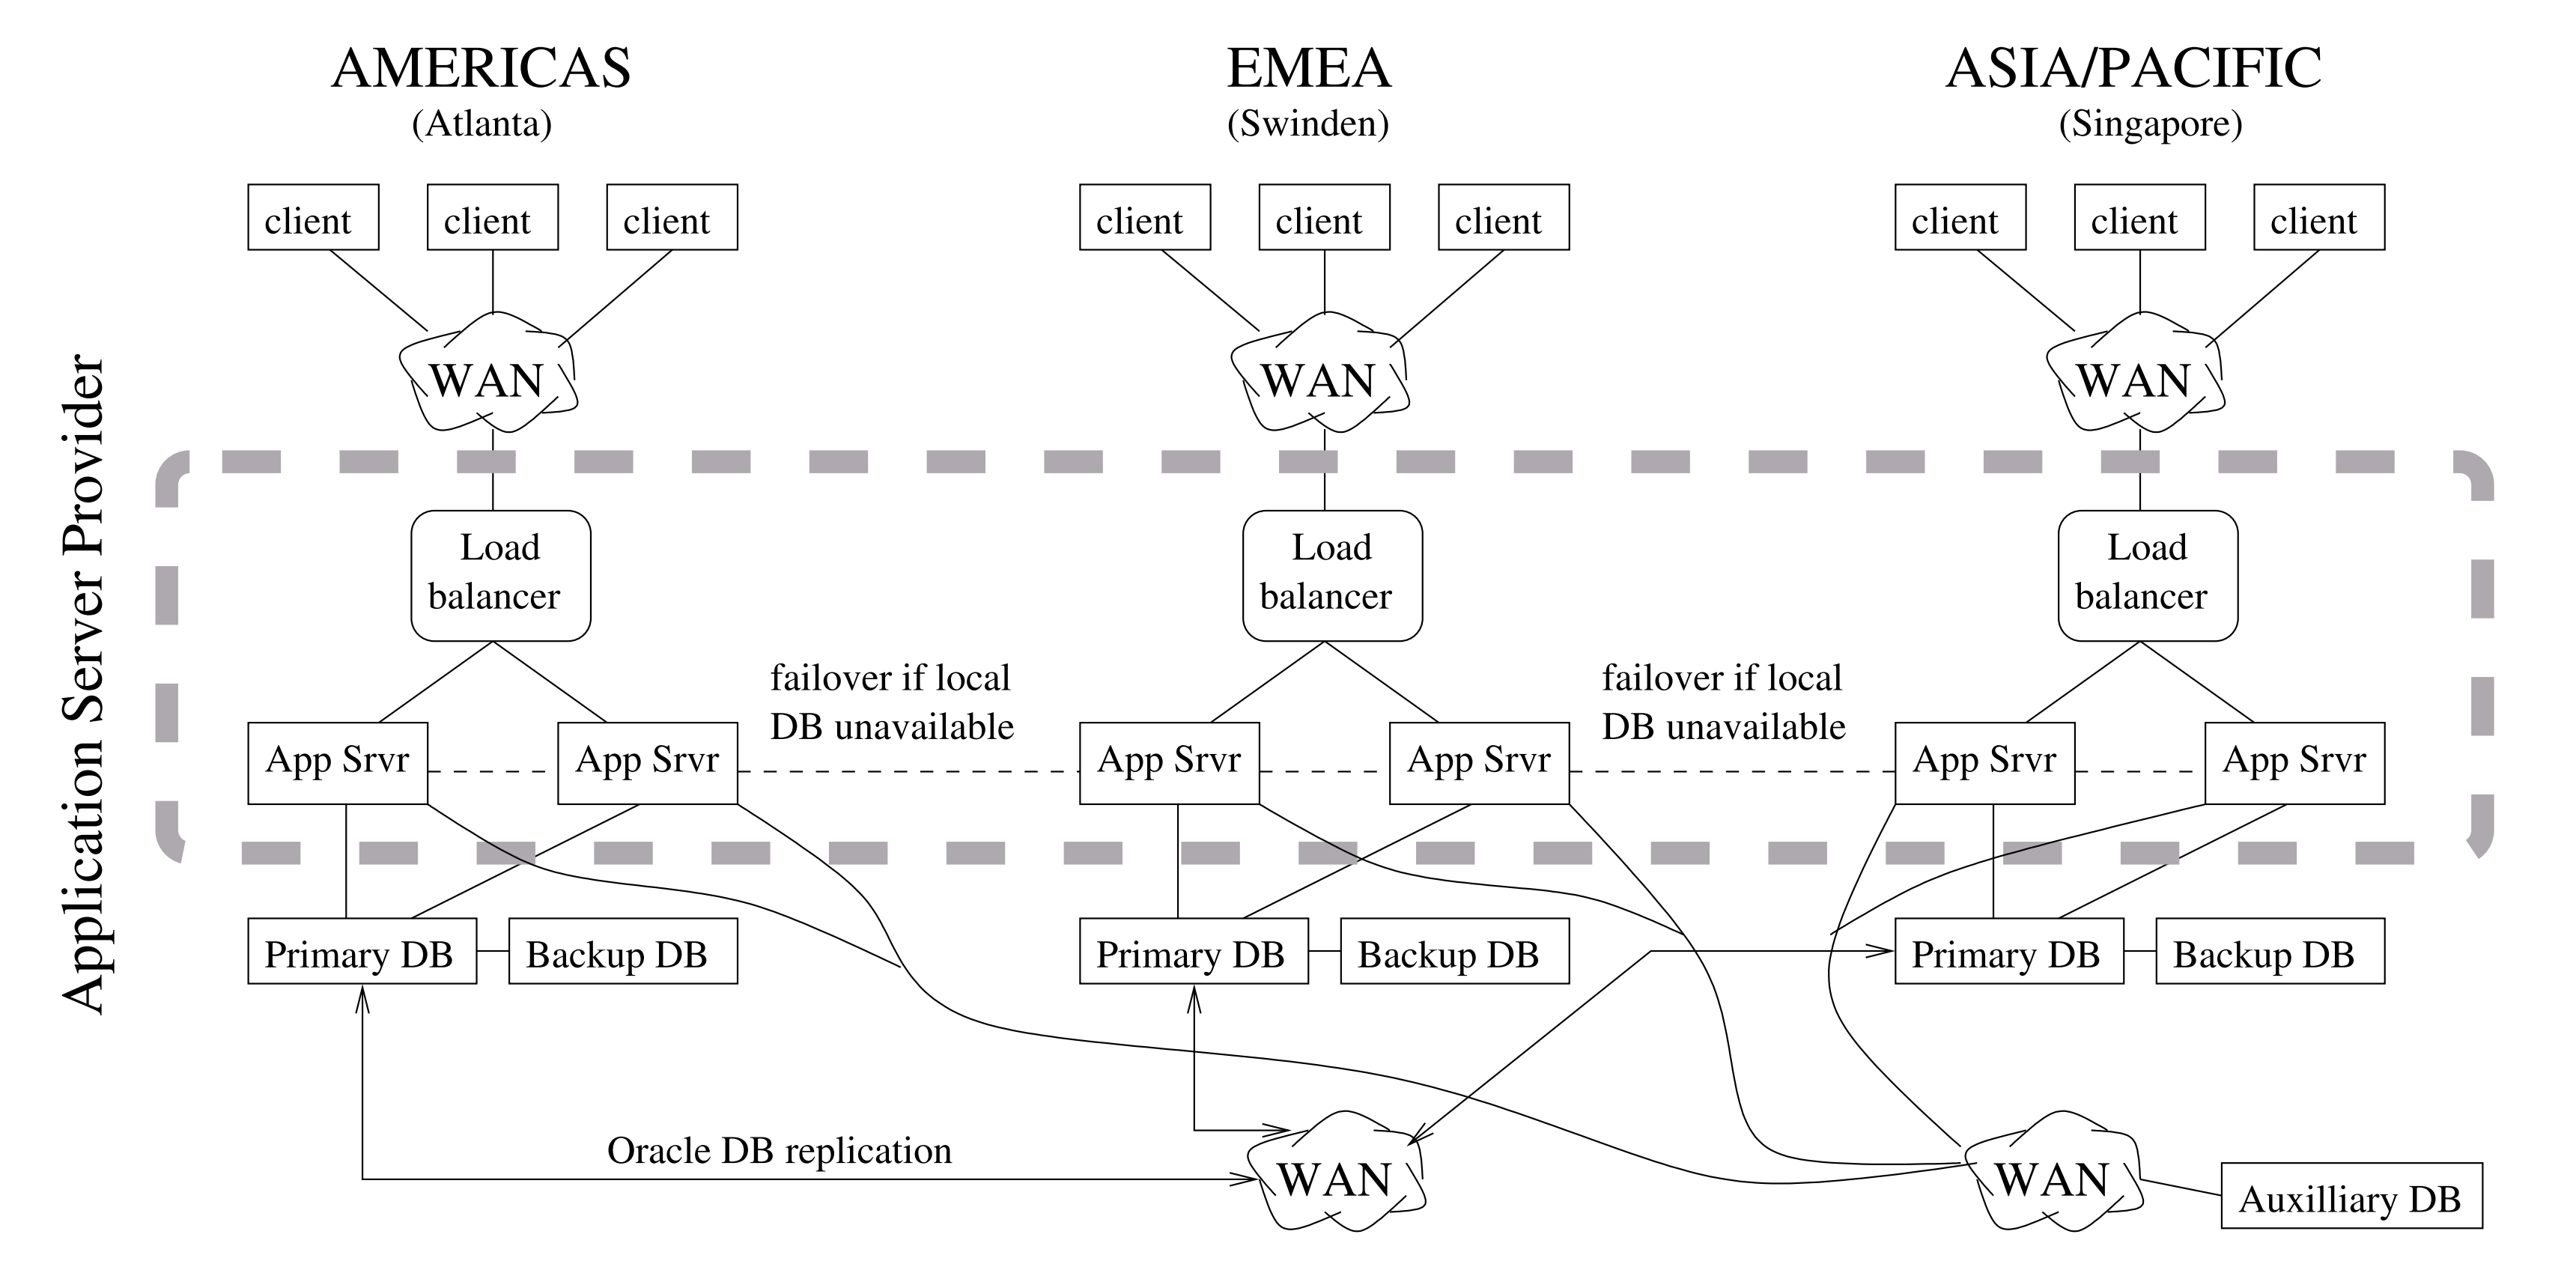
\includegraphics[width=10cm]{./app_provider.png}
  \end{figure}

\section{Weak point of the document}
\subsection{Metric Attribution and Ensembles Accuracy are not well discussed as in \cite{zhang2005ensembles}}
In this paper, all the different metrics are cross-validated for their contribution to ensemble accuracy using the following algorithm:

\begin{figure}[htbp]
  \centering
  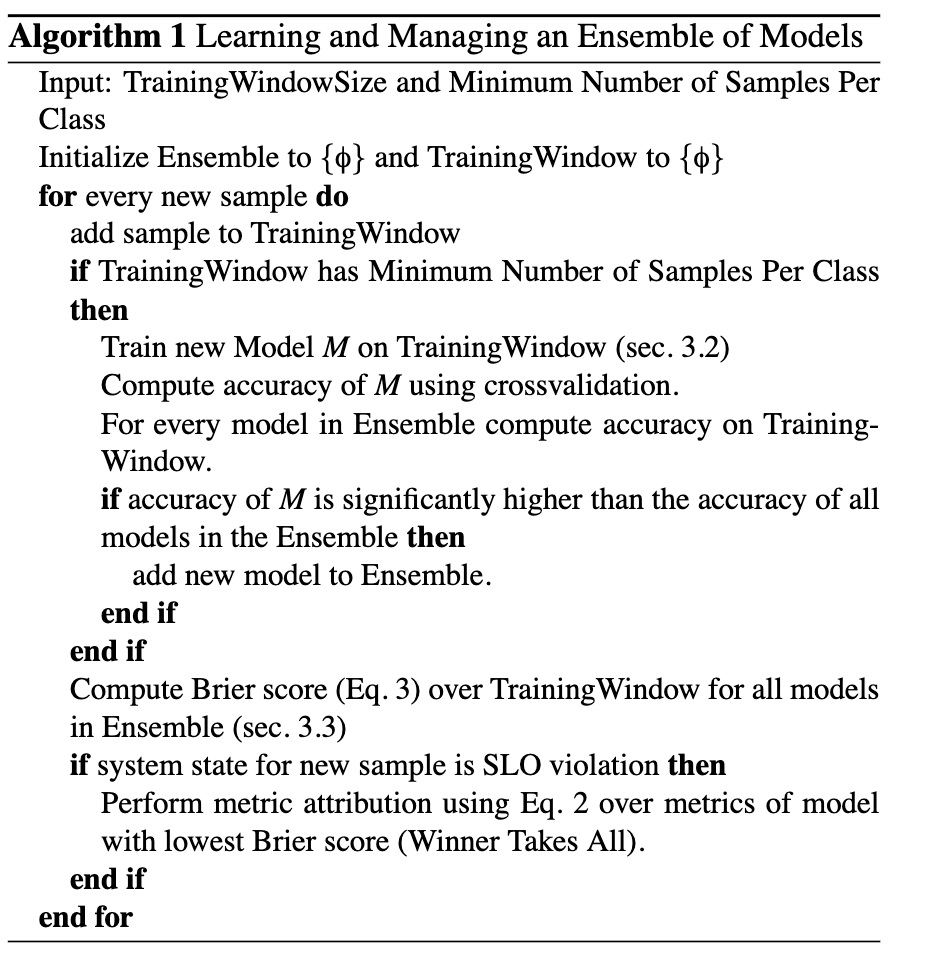
\includegraphics[width=8cm]{./cross_validate.png}
\end{figure}
\subsection{The metrics are not able to get the root of cause}
Whether the root of cause is memory leakage or network shutdown is not possible collected by pure observation.(with machine learning tools, it can be done now with fully automated tool). More expert enhanced knowledge is required to trigger a faulty state cause.
\subsection{Clustering Algorithm may cause no meaningful or too generic ensemble}
The $L_{1/2}$ norm algorithm is good for distinct normal/abnormal states, but not able to embed root causing knowledge to the state.
\section{Possible Refinement to the idea}
\subsection{Give a more detailed data illustration and mining to the SLO for root cause investigation\cite{wang2018cloudranger}}
\begin{figure}[htbp]
  \centering
  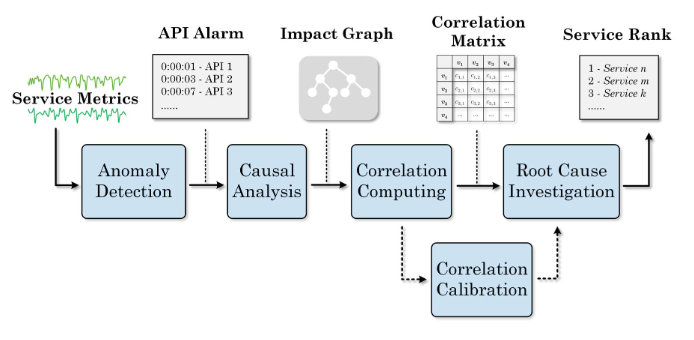
\includegraphics[width=8cm]{./cloudranger.png}
\end{figure}
In CloudRanger, it has the trace of the impact graph, it is to describe the impact relation between service sets, which is better for finding root of cause.
\bibliographystyle{ACM-Reference-Format}
\bibliography{capturing_indexing_clustering_and_retrieving_system_history}
\end{document}
\endinput
%%
%% End of file `sample-acmlarge.tex'.
